\chapter{Integration in a Neo4j}

In this section it is described how "Customizable Contraction Hierarchies" CCH is integrated into Neo4j. CCH arguments the input graph, which means it inserts arcs, so called shortcuts, that do not belong to the original data. To keep the change to the input graphs as little as possible we decided to not insert any arc into the graph that is stored inside the neo4j database, but introduce another graph data structure, the index graph. This index graph has an mapping to the input graph that is held by the database, by inserting two properties into the node of the input graph. The \textit{rank} this vertex has in the index graph and the \textit{indexing weight} it had during the last customization process. This gives yet another two advantages. One is that we get full control about the graph representation which is helpful to efficiently store and read the index graph for the disk. Another is that the with this approach it makes it easier to later on port the idea to another graph database manufactures.

\section{Index Graph Data Structure}

The index graph data structure is neither a adjacency list nor adjacency matrix. There is a vertex object that has two hash tables. One for incoming arc and one for outgoing arcs. The hash tables keys are of type vertex and the value is the arc. An arc has a reference to its start vertex and one to its end vertex. \\
A disadvantage of this model could be that some modern hardware optimization that exist for arrays do not match with this data structure. When using an array, the values this array are stored sequentially in main memory. When one value of an array is accessed by the CPU, modern hardware reads subsequent values into the CPU-cache because it is likely that they are accessed right after it. The model of the index graph is a linked data structure, a bit like a linked list. The elements of an linked list are contained somewhere in main memory. There is no guarantee that subsequent values have any spacial proximity. Therefore the just explained hardware optimization will not give any advantage. \\ % cite some paper to this topic
However, this makes the makes the graph traversal easy. Additional it makes it very efficient to explore the neighborhood of a vertex. There is no array traversal to find a vertex and only one hash table lookup for finding an arc of a vertex. Additionally these hash tables only contain few elements. This makes this data structure efficient anyway. Test on small graphs [Oldenburg] show that cch queries can be answered in less than one millisecond, which is close to what we tested with the original cch application.

\section{The mapping}

\begin{figure}
    \centering
    \begin{tikzpicture}[node distance={15mm}, main/.style = {draw, circle}]
 
    \node[main, align=center] (x3) at (0,4) {id:23, labels:\{\\Location,…\}, \\props:\{\\rank:3,…\}};
    \node[main, align=center] (x2) at (12,2) {id:22, labels:\{\\Location,…\}, \\ props:\{\\rank:2,…\}};
    \node[main, align=center] (x1) at (6, 0) {id:21, labels:\{\\Location,…\},  \\ props:\{\\rank:1,…\}};
    
    \draw[ -Stealth] (x2) -- node[rectangle,draw, fill=white,  align=center] {:ROAD \\ weight:1.0}(x1);
    \draw[ -Stealth] (x1) -- node[rectangle,draw, fill=white,  align=center] {:ROAD \\ weight:1.0} (x3);
    \draw[dashed, -Stealth] (x2) -- (x3);

    \draw (0,-2) -- (10,-2);
    \draw (0,-2.5) -- (10,-2.5);
    \draw (0,-3) -- (10,-3);
    \draw (0,-3.5) -- (10,-3.5);
    \draw (0,-4) -- (10,-4);

    \draw (0,-2) -- (0,-4);
    \draw (2.5,-2) -- (2.5,-4);
    \draw (5,-2) -- (5,-4);
    \draw (7.5,-2) -- (7.5,-4);
    \draw (10,-2) -- (10,-4);

    \node[align=center] at (1.25, -2.25) {\textbf{start rank}};
    \node[align=center] at (3.75, -2.25) {\textbf{end rank}};
    \node[align=center] at (6.25, -2.25) {\textbf{middle rank}};
    \node[align=center] at (8.75, -2.25) {\textbf{weight}};

    \node[align=center] at (1.25, -2.75) {2};
    \node[align=center] at (3.75, -2.75) {3};
    \node[align=center] at (6.25, -2.75) {1};
    \node[align=center] at (8.75, -2.75) {2.0};

    \node[align=center] at (1.25, -3.25) {1};
    \node[align=center] at (3.75, -3.25) {3};
    \node[align=center] at (6.25, -3.25) {-1};
    \node[align=center] at (8.75, -3.25) {1.0};

    \node[align=center] at (1.25, -3.75) {2};
    \node[align=center] at (3.75, -3.75) {1};
    \node[align=center] at (6.25, -3.75) {-1};
    \node[align=center] at (8.75, -3.75) {1.0};

\end{tikzpicture}
    \caption{mapping}
    \label{fig:mapping}
\end{figure}

\section{The Contraction}

\section{How to Store the Index Graph}

\begin{figure}
    \centering
    \begin{tikzpicture}[node distance={15mm}, main/.style = {draw, circle}]
    
    \draw (-7,6) rectangle (-1,7);
    \draw (-5.5,6) -- (-5.5,7);
    \draw (-4,6) -- (-4,7);
    \draw (-2.5,6) -- (-2.5,7);
    \node at (-6.25, 6.5) {from};
    \node at (-4.75, 6.5) {to};
    \node at (-3.25, 6.5) {middle};
    \node at (-1.75, 6.5) {weight};

    \draw [decorate,decoration = {brace, amplitude=5pt}] (-7,7.1) --  (-5.5,7.1);
    \draw [decorate,decoration = {brace, amplitude=5pt}] (-5.5,7.1) --  (-4,7.1);
    \draw [decorate,decoration = {brace, amplitude=5pt}] (-4,7.1) --  (-2.5,7.1);
    \draw [decorate,decoration = {brace, amplitude=5pt}] (-2.5,7.1) --  (-1,7.1);
    \node[ align=center] at (-6.25, 7.8) {32 bit  \\ integer};
    \node[ align=center] at (-4.75, 7.8) {32 bit  \\ integer};
    \node[ align=center] at (-3.25, 7.8) {32 bit  \\ integer};
    \node[ align=center] at (-1.75, 7.8) {32b bit \\ integer};

    \draw [decorate,decoration = {brace, amplitude=5pt}] (-1,5.9) --  (-7, 5.9);
    \node at (-4, 5.5) {16 byte DiskArc};

    \draw[dashed, -Stealth] (-1,7) -- (0, 6.7);
    \draw[dashed, -Stealth] (-1,6) -- (0, 6.3);
    
    
    \draw (0,7) -- (4,7);
    \draw[dashed] (0,6) -- (4,6);
    \draw[dashed] (0,5) -- (4,5);
    \node at (4.5,5) {0};
    \node at (4.5,1) {1};
    \draw (0,3) -- (5,3); 
    \draw[dashed] (0,2) -- (4,2);
    \draw[dashed] (0,1) -- (4,1);
    \draw[out=60, in=-120] (0,0) to (4, 0);
    \draw (0,0) -- (0,7); 
    \draw (4,0) -- (4,7); 
    \node at (2, 6.5) {DiskArc};
    \node at (2, 5.5) {DiskArc};
    \node[rotate=90, font=\Large] at (2, 4) {. . . . .};
    
    \node[rotate=-90] at (5.85, 5) {disk block};
    \draw [decorate,decoration = {brace, amplitude=10pt}] (5.2,7) --  (5.2,3);

    \node at (2, 7.2) {\textbf{Arc File}};

    %---------------------------------------------------------
    \draw (-7,0+1.5) -- (-1,0+1.5);
    \draw (-7,1+1.5) -- (-1,1+1.5);
    \draw (-7,-0.5+1.5) -- (-7,1+1.5);
    \draw (-5.5,-0.5+1.5) -- (-5.5,1+1.5);
    \draw (-4,-0.5+1.5) -- (-4,1+1.5);
    \draw (-2.5,-0.5+1.5) -- (-2.5,1+1.5);
    \draw[out=60, in=-120] (-1,0+1.5) to (-1,1+1.5);

    \node at (-6.25, 0.5+1.5) {37};
    \node at (-4.75, 0.5+1.5) {293};
    \node at (-3.25, 0.5+1.5) {73};
    \node at (-1.75, 0.5+1.5) {…};

    \node at (-8.5, 0.5+1.5) {disk block:};
    \node at (-8.5, -1+1.5) {rank:};
    \node at (-7, -1+1.5) {0};
    \node at (1.5-7, -1+1.5) {1};
    \node at (3-7, -1+1.5) {2};
    \node at (4.5-7, -1+1.5) {3};

    \draw [decorate,decoration = {brace, amplitude=5pt}] (-7,1.1+1.5) --  (1.5-7,1.1+1.5);
    \node[ align=center] at (0.75-7, 1.8+1.5) {32 bit  \\ integer};
    \node[ align=center] at (-4, 1.2+1.5) {\textbf{Position File}};
\end{tikzpicture}
    \caption{Disk Block}
    \label{fig:disk_block}
\end{figure}

\begin{figure}
    \centering
    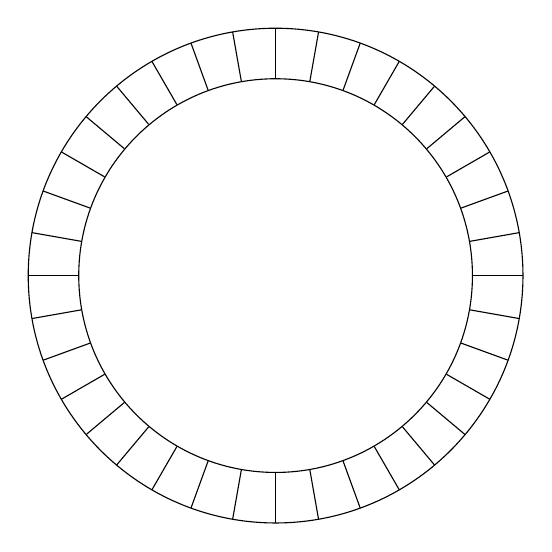
\begin{tikzpicture}[node distance={15mm}, main/.style = {draw, circle}]

    \draw (0,0) node[main, minimum size=5cm](z0) {} circle (pi);
    \draw (z0) -- (10:pi) node[midway,above]{};
    \draw (z0) -- (20:pi) node[midway,above]{};
    \draw (z0) -- (30:pi) node[midway,above]{};
    \draw (z0) -- (40:pi) node[midway,above]{};
    \draw (z0) -- (50:pi) node[midway,above]{};
    \draw (z0) -- (60:pi) node[midway,above]{};
    \draw (z0) -- (70:pi) node[midway,above]{};
    \draw (z0) -- (80:pi) node[midway,above]{};
    \draw (z0) -- (90:pi) node[midway,above]{};
    \draw (z0) -- (100:pi) node[midway,above]{};
    \draw (z0) -- (110:pi) node[midway,above]{};
    \draw (z0) -- (120:pi) node[midway,above]{};
    \draw (z0) -- (130:pi) node[midway,above]{};
    \draw (z0) -- (140:pi) node[midway,above]{};
    \draw (z0) -- (150:pi) node[midway,above]{};
    \draw (z0) -- (160:pi) node[midway,above]{};
    \draw (z0) -- (170:pi) node[midway,above]{};
    \draw (z0) -- (180:pi) node[midway,above]{};
    \draw (z0) -- (190:pi) node[midway,above]{};
    \draw (z0) -- (200:pi) node[midway,above]{};
    \draw (z0) -- (210:pi) node[midway,above]{};
    \draw (z0) -- (220:pi) node[midway,above]{};
    \draw (z0) -- (230:pi) node[midway,above]{};
    \draw (z0) -- (240:pi) node[midway,above]{};
    \draw (z0) -- (250:pi) node[midway,above]{};
    \draw (z0) -- (260:pi) node[midway,above]{};
    \draw (z0) -- (270:pi) node[midway,above]{};
    \draw (z0) -- (280:pi) node[midway,above]{};
    \draw (z0) -- (290:pi) node[midway,above]{};
    \draw (z0) -- (300:pi) node[midway,above]{};
    \draw (z0) -- (310:pi) node[midway,above]{};
    \draw (z0) -- (320:pi) node[midway,above]{};
    \draw (z0) -- (330:pi) node[midway,above]{};
    \draw (z0) -- (340:pi) node[midway,above]{};
    \draw (z0) -- (350:pi) node[midway,above]{};
    \draw (z0) -- (0:pi) node[midway,above]{};
    
\end{tikzpicture}
    \caption{Circular Buffer}
    \label{fig:circular_buffer}
\end{figure}
